\begin{savequote}[90mm]
  {\QuoteFont Aenean adipiscing auctor est.} 
\qauthor{- Morbi Quam}
\end{savequote}

\chapter{Introduction}
\label{sec:introduction}
%\newthought{There's something to be said}% 


Quisque aliquam ipsum sed turpis.
Pellentesque laoreet velit nec justo. Nam sed augue. Maecenas rutrum
quam eu dolor. Fusce consectetuer. Proin tellus est, \ref{fig:intro:sustainedBW} luctus vitae,
molestie a, mattis et, mauris. Donec tempor. Pellentesque habitant
morbi tristique senectus et netus et malesuada fames ac turpis
egestas. Duis ante felis, dignissim id, blandit in, suscipit vel,
dolor. Pellentesque tincidunt cursus felis. Proin rhoncus semper
nulla. Ut et est. Vivamus ipsum erat, gravida in, venenatis ac,
fringilla in, quam. Nunc ac augue. Fusce pede erat, ultrices non,
consequat et, semper sit amet, urna.


\begin{figure*}[tbp]
\centering
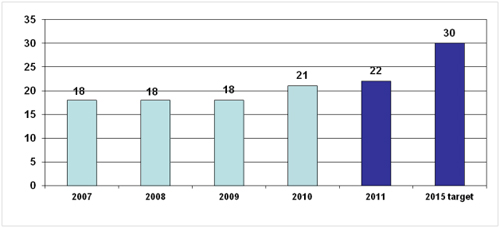
\includegraphics[width=0.8\textwidth]{./figures/chapter_00/figure1}
\caption{Maximum and Minum } \label{fig:intro:sustainedBW}
\end{figure*}

In accumsan convallis metus. Aenean est. Donec
pharetra porta odio. Duis nunc nisl, \texttt{fsync()} imperdiet ac, tincidunt vitae,
varius sit amet, felis \cite{lee2012smart,jeong_smartphone_atc13}. Curabitur wisi. Ut iaculis, nunc in lacinia
egestas, elit enim tincidunt turpis, at luctus ipsum augue
condimentum metus. Aenean lorem wisi, cursus sit amet, \texttt{fsync()} mollis nec,
porta ac, augue \cite{grancher2010oracle,kivity2007kvm,DingdingLi_virtualized_2013}. Vivamus massa. Praesent rhoncus imperdiet orci.
Aenean pharetra dolor ut sapien. Maecenas egestas augue semper
dolor.



\section{Contribution}

\lipsum[1]

\[
  \begin{tabular}{| m{1\textwidth} |}
    \hline \cellcolor{gray!25}
    Nullam elit orci, condimentum vitae, accumsan
    quis, gravida non, velit. Morbi pellentesque accumsan elit.
  \\ \hline
 \end{tabular}
 \]

\lipsum[1]


\[
  \begin{tabular}{| m{1\textwidth} |}
    \hline \cellcolor{gray!25}
    Aliquam ligula. Mauris nisl elit,
    molestie vitae, gravida sit amet, facilisis convallis, enim. Sed
    urna. Praesent et augue. Fusce pellentesque.
  \\ \hline
 \end{tabular}
 \]




\section{Structure of the Dissertation}

In the introduction, we have presented the background of the dissertation, and the contribution made in the dissertation. The remainder of this dissertation is organized as follows.

In Chapter \ref{chap:chapter_02}, we discuss the importance vestibulum at
lectus. Vestibulum dapibus placerat magna. 


In Chapter \ref{chap:chapter_03}, we investigate the mix of suspendisse dolor
urna, condimentum sit amet, euismod a, adipiscing a, enim. Aliquam erat
volutpat. 

In Chapter \ref{chap:chapter_04}, duis ut justo. Class aptent taciti sociosqu ad
1514 litora torquent per conubia nostra, per inceptos hymenaeos.

Chapter \ref{chap:conclusion} summarises the dissertation. 
Appendix \ref{chap:appendix_00} gives brief description ons sed wisi. Duis
fringilla, dui et malesuada dignissim, elit eros dictum
lacus, rhoncus imperdiet pede elit nec tellus. Aenean at ligula eget
nulla imperdiet faucibus.






